\documentclass[a4paper,14pt]{article}
\usepackage{fullpage}
\usepackage{times}
\usepackage{amssymb,amsthm,amsmath}
\usepackage{verbatim}
\usepackage{ctex}
\usepackage{bm}
\usepackage{graphicx}
\usepackage{enumerate}
\usepackage{url}
\usepackage{color}
\usepackage{geometry}
\usepackage{listings}
\geometry{a4paper,left=2cm,right=2cm,top=1cm,bottom=2cm}

\pagestyle{plain}
\title{Git版本控制软件和GitHub平台使用基础教程}
\author{有限元法基础助教:倪锐晨}
\begin{document}
\maketitle

自从高级语言Fortran被广泛使用,人类所开发的软件规模爆炸式地增长起来。随之而来的还有大型程序开发与维护中的许多严重问题,这些问题可能导致软件产品的寿命缩短,甚至夭折。这就是所谓的软件危机。人类在应对软件危机的过程中逐渐总结出一套方法,形成了软件工程这一学科。其中,一个非常重要的方法就是要对程序进行严格的版本控制。

其中,Git是一个分布式管理系统。这意味着每个开发者的计算机上都有一个完整的仓库,包括完整的源代码以及开发历史。每个开发者需要在自己的仓库内完成自己的工作,形成稳定版本后再上传至远程服务器。这大大减少了开发者之间的冲突,并且对网络的依赖也不如SVN那样严重。

因此,在本课程的学习过程中,我们将结合使用Git软件和GitHub平台对大作业的代码进行版本控制管理,并将使用Git协同工作的协同程度计入大作业的评分考量,希望大家熟悉并掌握基于版本控制的代码协同开发。

\section{Git的安装}
\subsection*{Linux系统}
打开终端,运行命令

sudo get-apt install git

即可安装Git。
\subsection*{Windows系统}
前往Git的官方下载网址(\url{https://git-scm.com/downloads}),选择Windows的版本下载软件安装包。下载完毕后双击运行软件安装包,一切都选择默认选项即可。安装完成后,在任意文件夹下单击鼠标右键,如果出现如图1所示的“Git Bash Here”和“Git GUI Here”则说明安装成功。
\begin{figure}[h]
\centering
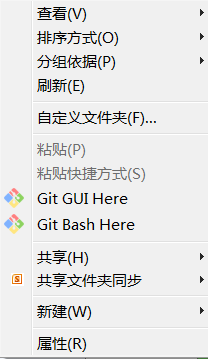
\includegraphics[height=6cm]{figure/Git_Success}
\caption{Git软件成功安装}
\end{figure}

\section{GitHub平台的注册和学生私有库权限的申请}
\subsection*{GitHub用户注册}
本学期的大作业代码将统一保存在GitHub平台上,为此需要先前往GitHub的官网(\url{https://github.com/})进行账号的注册:
\begin{enumerate}[1. ]
\item 在如图2所示的界面中填写自己的用户名、邮箱和密码。邮箱一定要使用清华大学的邮箱以申请学生私有库的权限,用户名推荐使用自己的名字全拼(例如助教倪锐晨的用户名可以设置为 Ruichen-Ni)以便老师和助教识别大家的身份。
\begin{figure}[h]
\centering
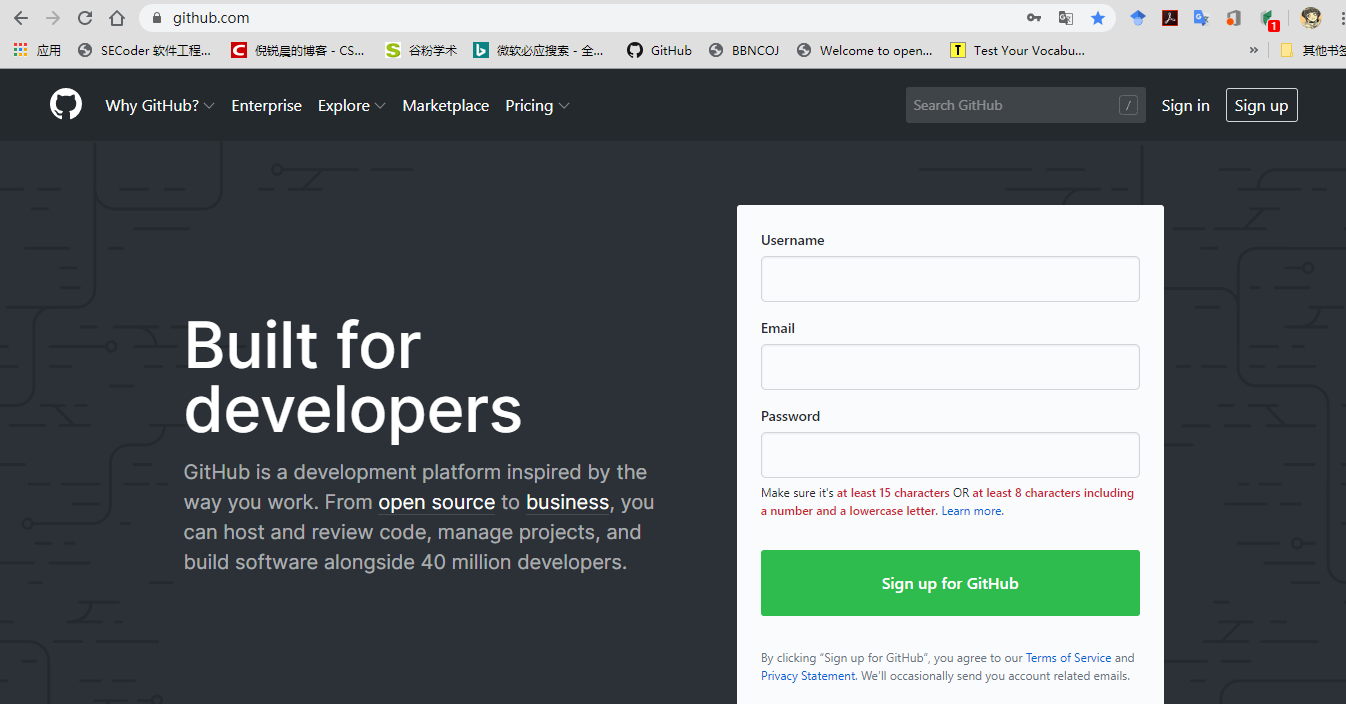
\includegraphics[height=7cm]{figure/GitHub_SignUp}
\caption{GitHub平台注册界面}
\end{figure}
\item GitHub会进入一个人机识别界面,正常操作即可,如图3所示
\begin{figure}[h]
\centering
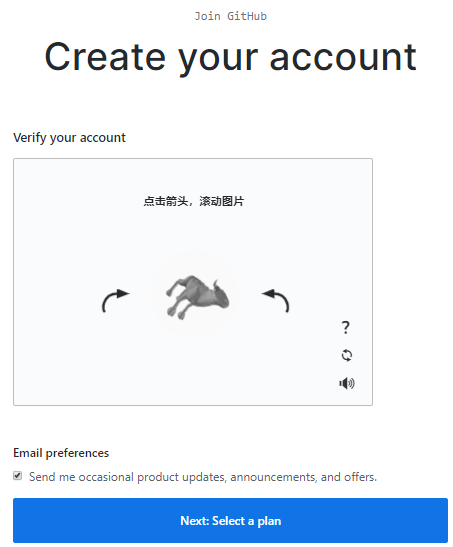
\includegraphics[height=7cm]{figure/Compute_Verify}
\caption{GitHub平台人机识别}
\end{figure}
\newpage
\item GitHub会让大家选择一个账号计划(plan),我们选择左边的Free Plan即可,如图4所示
\begin{figure}[h]
\centering
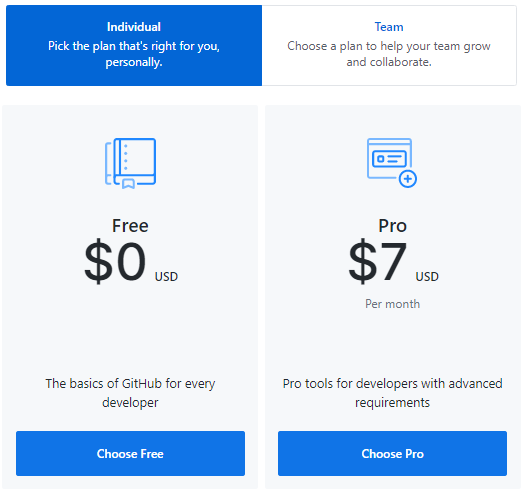
\includegraphics[height=6cm]{figure/Plan_Select}
\caption{GitHub平台账户计划选择}
\end{figure}
\item GitHub平台会让大家填写一个用户问卷,大家可以按照自己的情况填写,也可以将网页拉到最下面选择跳过此步骤。大家打开邮箱后点击账户激活链接即可完成GitHub账号的申请,如图5所示
\begin{figure}[h]
\centering
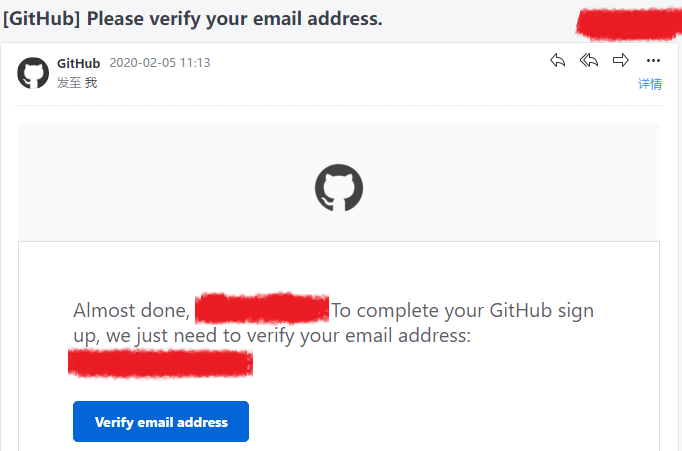
\includegraphics[height=5cm]{figure/Verify_mail}
\caption{GitHub平台账号激活邮件}
\end{figure}
\item 可以通过GitHub的登录界面(\url{https://github.com/login})进行登录,如图6所示
\begin{figure}[h]
\centering
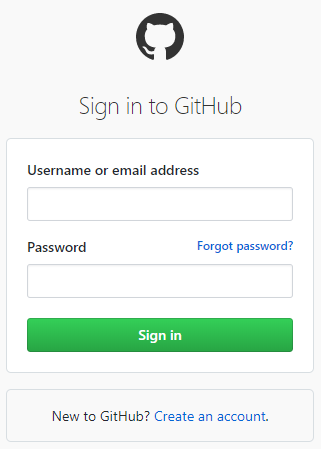
\includegraphics[height=5cm]{figure/GitHub_SignIn}
\caption{GitHub平台登录界面}
\end{figure}
\end{enumerate}
\newpage

\quad

\quad

\subsection*{学生免费私有库权限申请}
大作业会进行分组,为了保证各组独立完成该训练模块,我们要求大作业的代码仓库是私有的。同时每个组需要将老师和助教的账号也加入到自己的组内以便我们进行大作业进程的监督和最后的打分。GitHub的Free plan对于private的代码仓库只允许三个合作者,不满足我们课程的需求。因此需要在GitHub平台上申请学生私有库权限,申请后private的代码仓库允许无限多的合作者(每个组的组长必须申请以邀请组内成员,其他同学可以按照自己的情况决定是否申请)。
\begin{enumerate}[1. ]
\item 前往GitHub的教育申请界面(\url{https://education.github.com/students}),如图7所示,点击图中的“Get benefits for students”按钮。如果网页显示打不开,请通过SSLVPN挂回清华的IP地址(我家的网络IP地址就无法登陆该网站)。
\begin{figure}[h]
\centering
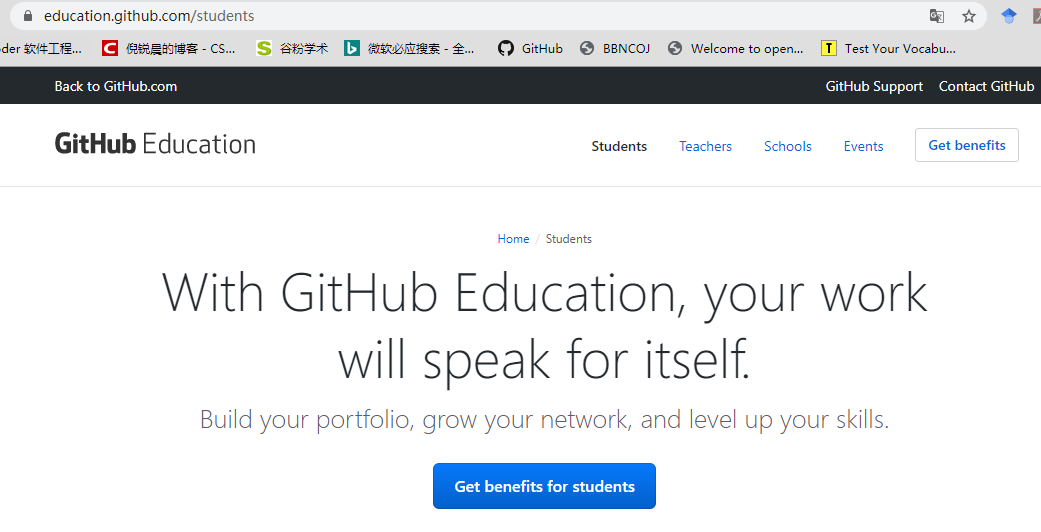
\includegraphics[height=6cm]{figure/GitHub_Edu}
\caption{GitHub平台学生权限申请}
\end{figure}
\item 进入到如图8所示的界面,如实填写个人信息。由于GitHub平台会检测申请发出的地理位置,不在学校附近的话申请会被拒绝。因此我们需要提供额外信息:将学生证照片和清华大学公众号的防疫通报截图合成在同一图片内上传(因为只允许上传一张照片),并在描述申请用途中写清楚“自己是清华大学学生,这次申请是为了进行有限元课程的学习,并且清华大学因为疫情决定在家通过远程MOOC在线上课”(由于是人工审核的,请大家自行翻译上面的这段话,意思相近即可,完全一致容易被误认为是机器申请而被拒绝)。然后点击“Submit your information”按钮即可
\begin{figure}[h]
\centering
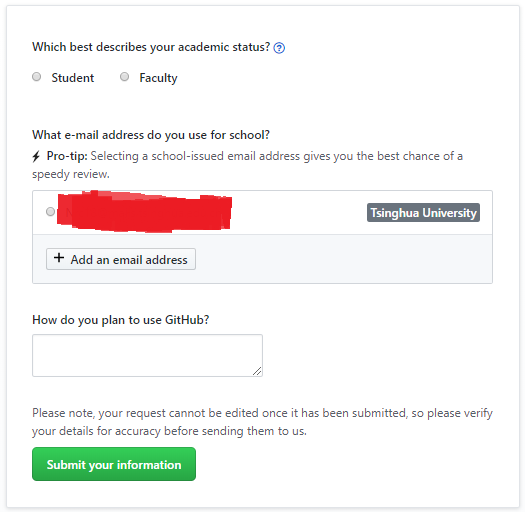
\includegraphics[height=6cm]{figure/GitHub_Edu_Apply}
\caption{GitHub平台学生权限申请问卷}
\end{figure}
\newpage
\item 几个工作日内,GitHub会向通过申请的账号邮箱发送如图9所示的申请成功邮件
\begin{figure}[h]
\centering
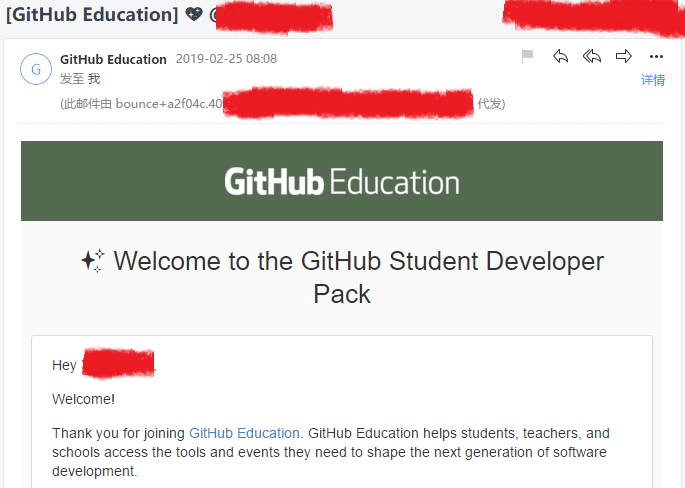
\includegraphics[height=6cm]{figure/GitHub_Edu_mail}
\caption{GitHub平台学生权限申请成功邮件}
\end{figure}
\item 如果第一次申请被拒绝,GitHub会发送申请失败邮件,查看失败原因补充相关材料后发起第二次申请
\begin{figure}[h]
\centering
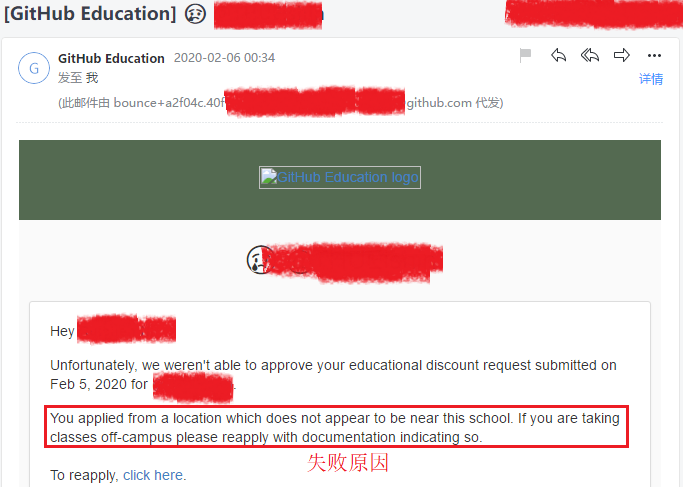
\includegraphics[height=6cm]{figure/GitHub_Edu_mail_f}
\end{figure}
\item 如果一直没有收到邮件,可以重新进入申请界面,申请界面右侧会有你的申请记录,如下图所示
\begin{figure}[h]
\centering
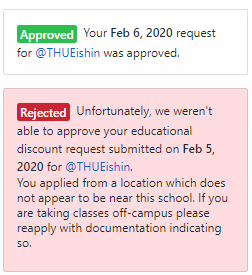
\includegraphics[height=5cm]{figure/1}
\end{figure}
\end{enumerate}

\newpage

\quad

\quad

\quad

\section{Git和GitHub的“Hello, World!”}
任何语言的学习都会以一个“Hello, World!”程序进行入门学习,Git也不例外。在这里我们会以一个简单的例子来讲解GitHub平台SSH Key的配置、代码仓库(repository)的创建、主分支(branch master)的合并保护权限的设置、本地仓库的创建、本地分支的创建、本地分支的提交、本地分支的合并、本地仓库向远端仓库推送、远端仓库的分支合并以及冲突处理。

\quad

\subsection*{SSH Key的设置}
如果不使用SSH Key,每次向远端仓库提交时都会要求输入用户名和密码以确认用户的身份。配置了SSH Key之后,就免去了用户名和密码匹对的过程,在我们使用git push命令时会自动进行本地私钥和远端公钥的匹配,从而避免了输入用户名和密码的重复工作。
\begin{enumerate}[1. ]
\item 在任意文件夹下点击鼠标右键打开“Git Bash Here”进入Git的命令行界面,如图10所示(我是在/e/temp文件夹下进行的),输入如下命令

ssh-keygen -t rsa -C "your email"

用你注册GitHub账号时使用的邮箱代替命令中的your email,询问文件名称时推荐修改默认文件名(我使用的是 ./id\_rsa\_github)以便多账号的使用(没有多账户的同学也可以选择直接使用系统默认的文件名),询问私钥文件密码时可以选择不输入直接回车以方便以后推送,也可以选择设置以增加安全性。
\begin{figure}[h]
\centering
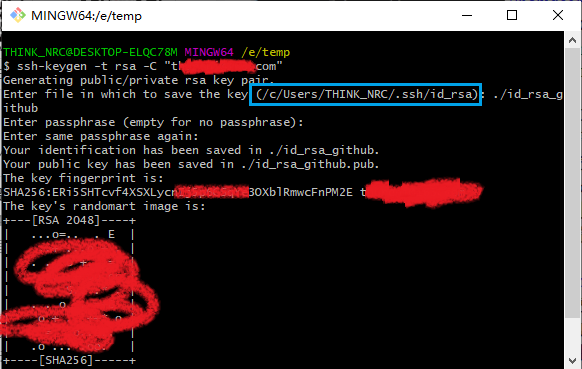
\includegraphics[height=6cm]{figure/sshkey}
\caption{SSH Key生成}
\end{figure}

将生成的私钥文件和公钥文件拷贝到Git可以访问的文件夹下,即询问文件名时系统提供的绝对路径(图中蓝框位置处,本例中为/c/Users/THINK\_NRC/.ssh/)。如果没有该文件夹就创建一个。

\newpage

\quad

\quad

\quad

\item 使用注册的账号登录GitHub平台,点击界面右上方的头像下拉菜单进入“settings”选项卡,在settings选项卡选择“SSH and GPG keys”选项,如图11所示。点击图中的“New SSH key”按钮。
\begin{figure}[h]
\centering
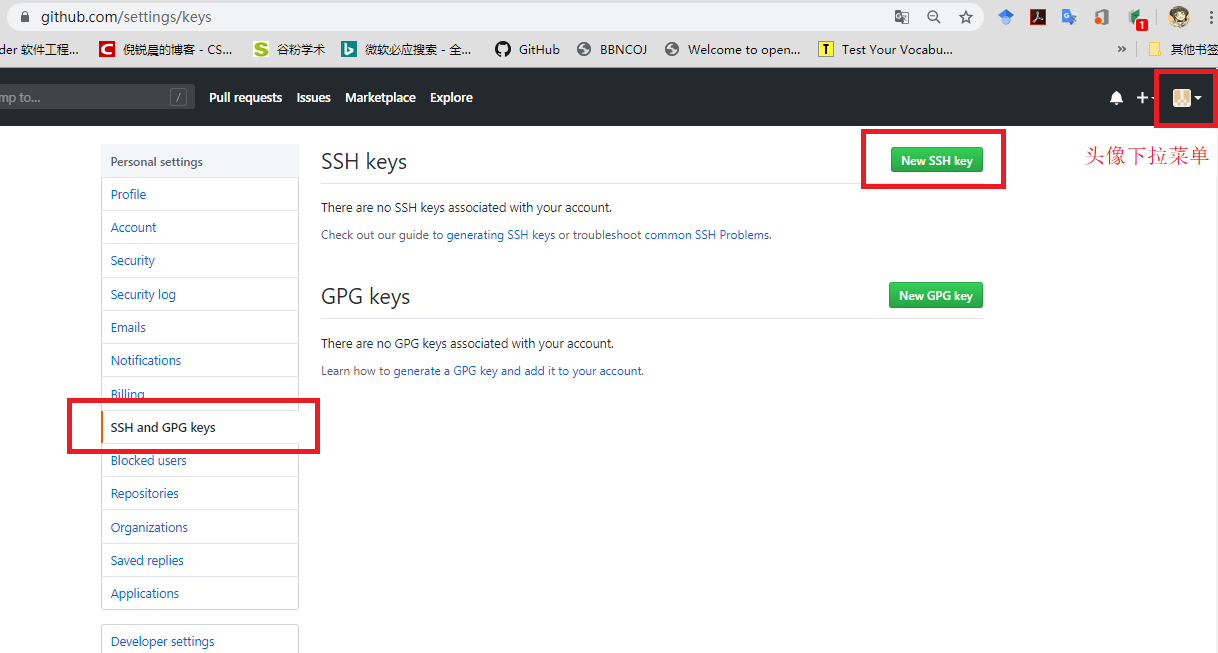
\includegraphics[height=7cm]{figure/GitHub_settings}
\caption{SSH Key公钥设置}
\end{figure}
\item 打开公钥(.pub)文件,复制所有内容粘贴到图12所示的“Key”框内,在Title框内随便取一个易辨别的名字(例如Windows系统产生的公钥就命名为Windows),点击“Add SSH key”按钮即可。
\begin{figure}[h]
\centering
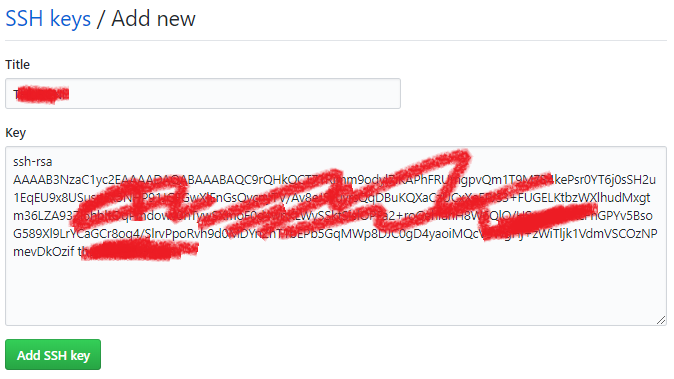
\includegraphics[height=7cm]{figure/SSHSet}
\caption{SSH Key公钥设置2}
\end{figure}
\end{enumerate}

\newpage

\quad

\quad

\quad

\subsection*{GitHub私有仓库的创建和配置}
\begin{enumerate}[1. ]
\item 点击右上方头像左边的加号“+”的下拉菜单,选择其中的“New Repository”选项,出现如图13所示的新建仓库页面。“Repository name”是必须的,请选择一个能够反映仓库作用的名字。“Description”也尽可能描述清楚仓库的作用。仓库属性选择“Private”。勾选“README”文件创建的选项,该README文件可用于记录每个组员向大作业代码中添加的功能。根据大作业代码的语言选择.gitignore文件以排除相关工程文件的提交。全部设置完毕后点击“Create repository”按钮。
\begin{figure}[h]
\centering
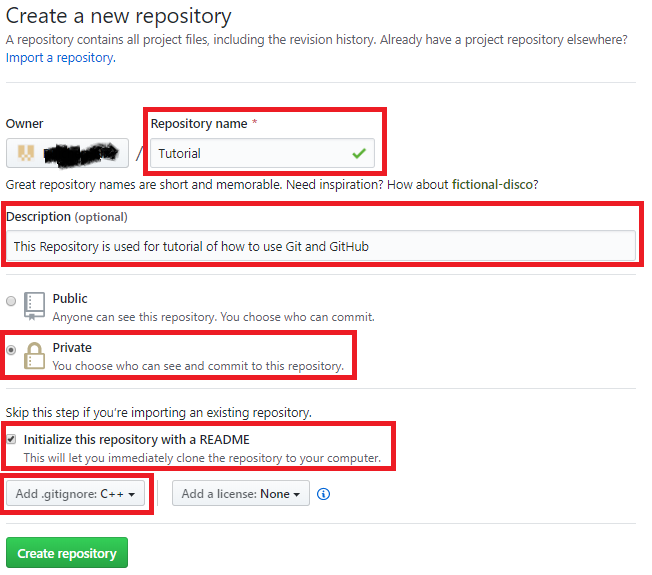
\includegraphics[height=14cm]{figure/Repository}
\caption{GitHub私有仓库的创建}
\end{figure}
\newpage

\quad

\quad

\quad

\item 进入新建仓库“settings”选项卡下的“Collaborators”选项,如图14所示。在下方的搜索框内搜索组员的GitHub用户名,搜到后可以点击“Add collaborator”按钮向组员发出加入仓库的邀请,组员会收到邀请邮件,选择接受邀请就可以对仓库代码进行协同开发。
\begin{figure}[h]
\centering
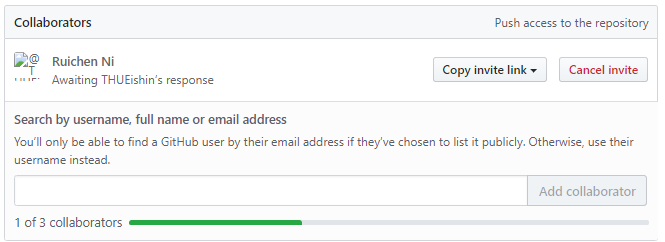
\includegraphics[height=5cm]{figure/collab}
\caption{GitHub私有仓库成员邀请}
\end{figure}
\item 进入新建仓库“settings”选项卡下的“Branches”选项,如图15所示。点击图中的“Add rule”按钮。(私有仓库必须通过学生权限申请后才能添加分支权限设置。)
\begin{figure}[h]
\centering
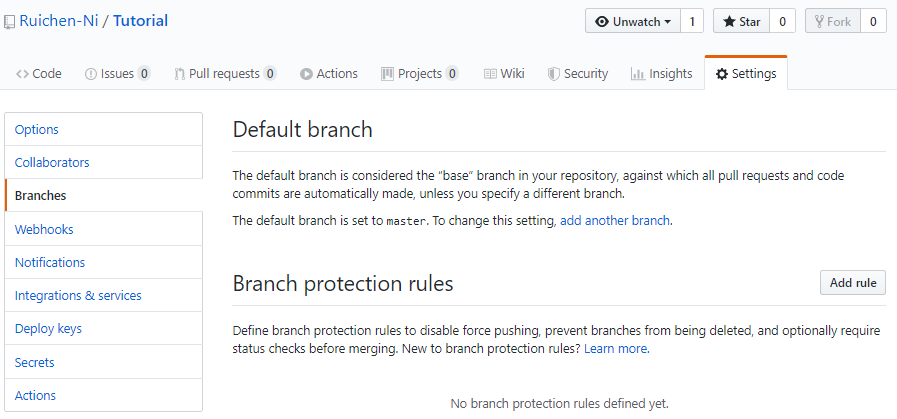
\includegraphics[height=7cm]{figure/branch_rule_set}
\caption{GitHub仓库的分支权限设置}
\end{figure}
\newpage
\quad

\quad

\quad

\item 在分支权限设置页面请按图16所示设置。其中“Required approving reviews”推荐设置为2或者3,即至少组长和组内另外一位成员查看代码后认为没有问题才允许向master分支合并以增强master分支的稳定性。另外,“Rules applied to everyone including administration”中的两个选项绝对不能勾选以避免软件危机的出现。
\begin{figure}[h]
\centering
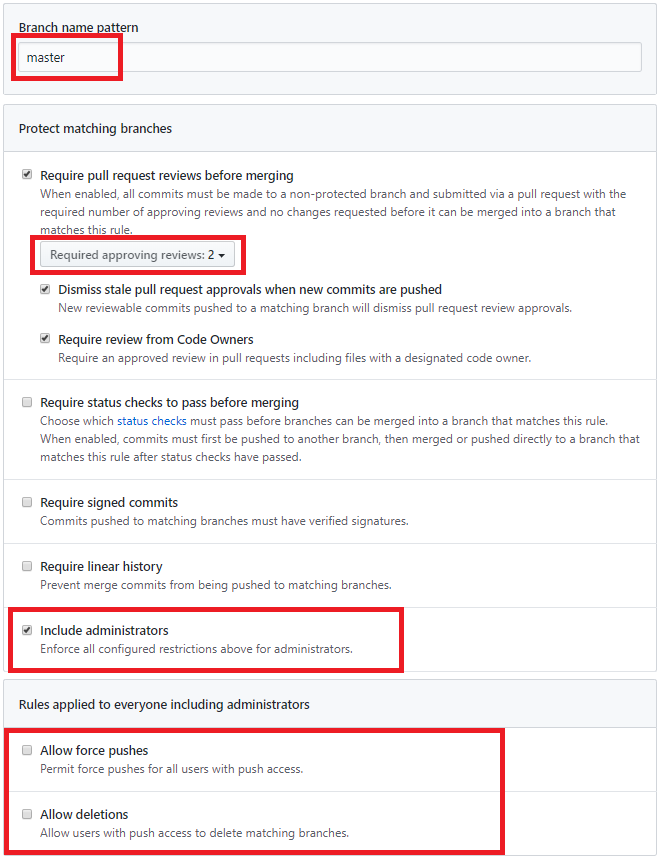
\includegraphics[height=18cm]{figure/branch_rule2}
\caption{GitHub仓库分支权限设置}
\end{figure}
\end{enumerate}


\newpage
\subsection*{一个简单的例子}

假设现在来了一个任务:需要从零开发出软件Tutorial的1.0版本,该版本包含两个功能feature1和feature2,这两个功能将分别由同学A和同学B完成(在本例中我会用两个账号来演示这个例子)。

先来看A同学完成feature1的开发:
\begin{enumerate}[1. ]
\item 新建一个空的文件夹(本例中为/e/temp/),进入文件夹内单击鼠标右键选择“Git Bash Here”打开Git的命令行窗口。如图17所示,在命令行窗口中输入如下命令初始化本地仓库

{\color{red}
\begin{lstlisting}[language=C]
git init
\end{lstlisting}
}
\begin{figure}[h]
\centering
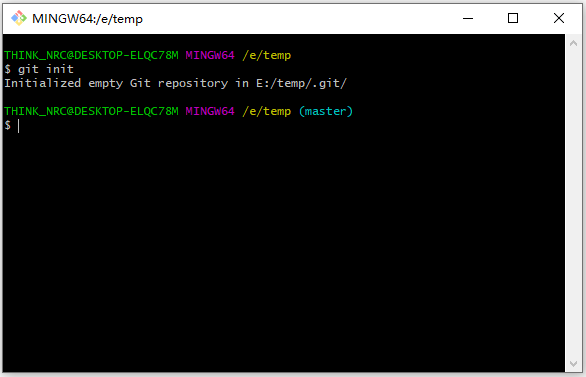
\includegraphics[height=6cm]{figure/step1}
\caption{本地仓库初始化}
\end{figure}
\item 为项目配置用户名和邮箱

单独为本项目配置:

{\color{red}
\begin{lstlisting}[language=C]
git config  user.email "GitHub注册邮箱"
\end{lstlisting}
}

{\color{red}
\begin{lstlisting}[language=C]
git config  user.name "GitHub用户名"
\end{lstlisting}
}

为电脑内所有项目配置用户名和邮箱

{\color{red}
\begin{lstlisting}[language=C]
git config  --global user.email "GitHub注册邮箱"
\end{lstlisting}
}

{\color{red}
\begin{lstlisting}[language=C]
git config  --global user.name "GitHub用户名"
\end{lstlisting}
}
\begin{figure}[h]
\centering
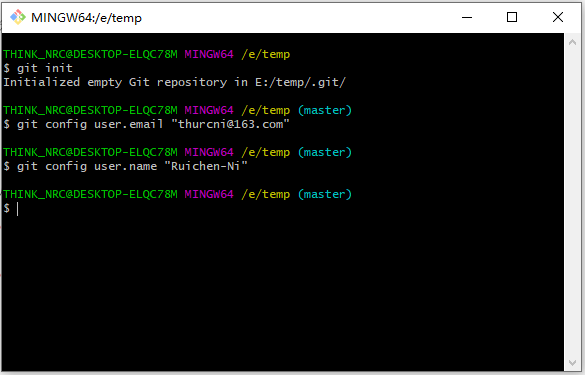
\includegraphics[height=6cm]{figure/step2}
\caption{配置用户名和邮箱}
\end{figure}

\newpage

\quad

\quad

\quad

\item 可以通过如下命令来查看本项目的配置,可以看到我们成功设置了用户名和邮箱
{\color{red}
\begin{lstlisting}[language=C]
git config  --local --list
\end{lstlisting}
}
\begin{figure}[h]
\centering
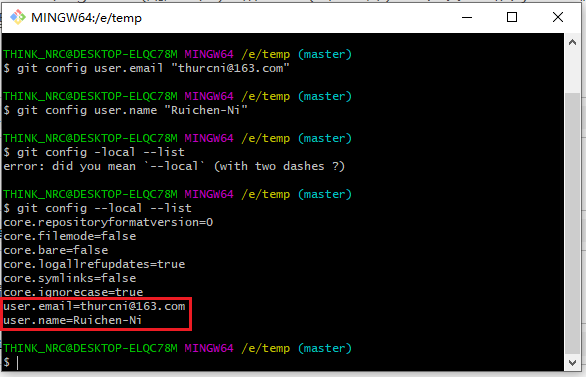
\includegraphics[height=6cm]{figure/step3}
\caption{查看项目配置}
\end{figure}

\item 点击图20中的“Clone or download”按钮,并点击“Use SSH”切换成如图所示的选项卡,复制其中的SSH仓库地址(本例中的仓库地址为git@github.com:Ruichen-Ni/Tutorial.git)
\begin{figure}[h]
\centering
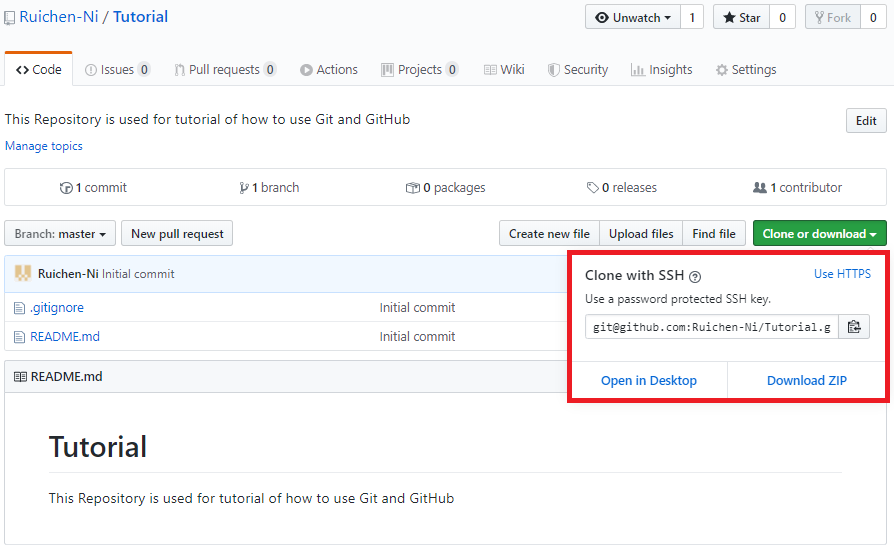
\includegraphics[height=7cm]{figure/repository_clone}
\caption{GitHub仓库的SSH地址}
\end{figure}

\newpage

\quad

\quad

\quad

\item 在Git的命令行窗口输入如下命令将远端仓库克隆到本地
{\color{red}
\begin{lstlisting}[language=C]
git clone 仓库地址
\end{lstlisting}
}
\begin{figure}[h]
\centering
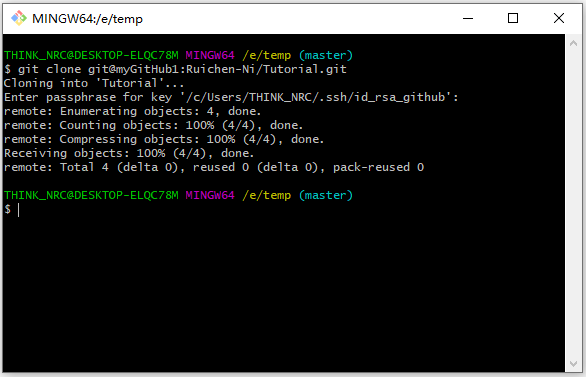
\includegraphics[height=6cm]{figure/step4}
\caption{GitHub仓库的克隆}
\end{figure}

\quad

\noindent 细心的同学会发现我输入的是git@myGitHub1:Ruichen-Ni/Tutorial.git而不是git@github.com:Ruichen-Ni/Tutorial.git。这是因为我有多个版本控制的账号,需要通过一个如图22的配置文件(该文件与私钥和公钥文件在同一文件夹下,并且该文件名为config,没有后缀名)来定位到底使用哪一个私钥文件。
\begin{figure}[h]
\centering
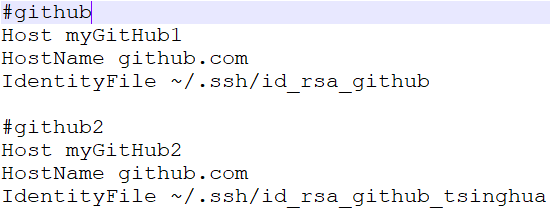
\includegraphics[height=5cm]{figure/config}
\caption{多个账户SSH Key的配置文件}
\end{figure}

\newpage
\item 为了开发Tutorial软件的1.0版本,A同学需要新建一个开发分支dev。进入Tutorial文件夹(可以直接在命令行窗口输入命令 {\color{red} cd Tutorial},也可以在文件管理器中进入Tutorial文件夹单击鼠标右键重新运行Git的命令行窗口),并输入如下命令(依次表示创建dev分支,切换到dev分支和查看分支状态)。前面带*号的分支表示目前所在的分支。

{\color{red}
\begin{lstlisting}[language=C]
git branch dev
git checkout dev
git branch
\end{lstlisting}
}
\begin{figure}[h]
\centering
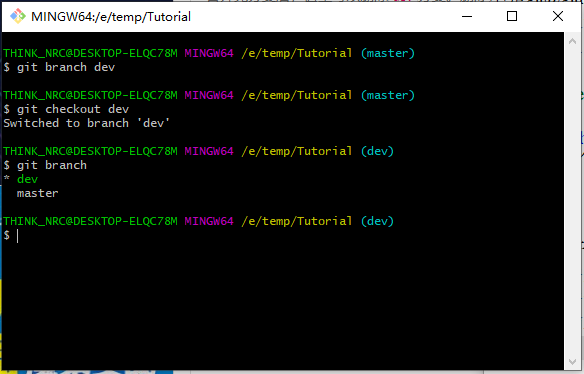
\includegraphics[height=6cm]{figure/step5}
\caption{创建分支、切换分支和查看分支状态}
\end{figure}

\item A同学通过如下的命令在GitHub远端仓库同时创建了一个对应的dev分支用于软件开发
{\color{red}
\begin{lstlisting}[language=C]
git push origin dev:dev
\end{lstlisting}
}

\begin{figure}[h]
\centering
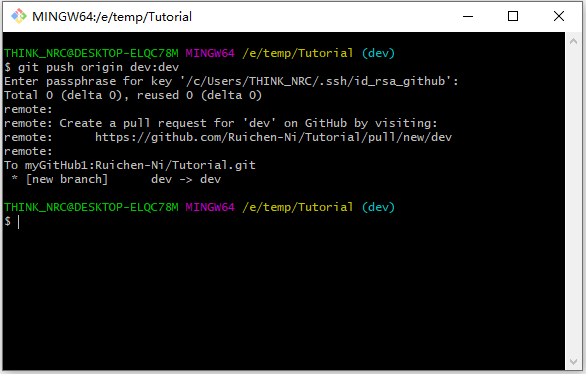
\includegraphics[height=6cm]{figure/step6}
\caption{创建GitHub远端仓库的开发分支dev}
\end{figure}
\newpage
\item A同学现在开始着手开发功能feature1,他需要从dev分支上创建一个分支fea1用于功能的开发,类似上面创建dev分支的操作,这里给出相应的命令但不再赘述。
{\color{red}
\begin{lstlisting}[language=C]
git branch fea1
git checkout fea1
git push origin fea1:fea1
\end{lstlisting}
}
\item A同学添加了一个文件名为feature1.txt的文件代表功能feature1的开发完成,可以通过如下命令进行工作区状态的检测和向本地仓库提交修改
{\color{red}
\begin{lstlisting}[language=C]
touch feature1.txt
git status
git add -A
git commit -m "Finish Feature 1"
\end{lstlisting}
}

\begin{figure}[h]
\centering
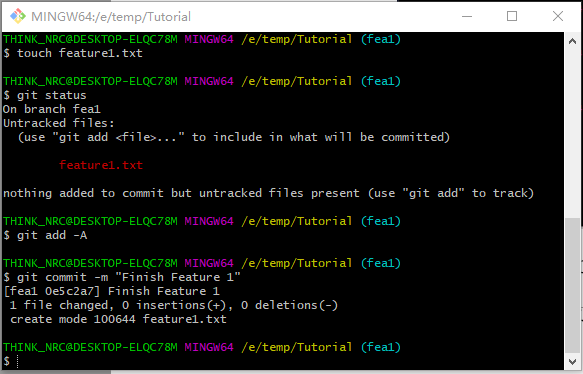
\includegraphics[height=6cm]{figure/step7}
\caption{文件修改、工作区状态检测、将修改提交至缓存区和将修改提交至本地仓库}
\end{figure}
\item A同学将完成的功能feature1的相关代码通过如下的代码提交到GitHub远端库。登录A同学的GitHub账号会发现系统提醒我们有fea1分支上存在新的提交并提示我们进行比较合并。当A同学检查觉得功能feature1的代码正确无误就可以点击“Compare \& pull request”按钮发起Pull Request。
{\color{red}
\begin{lstlisting}[language=C]
git push origin fea1:fea1
\end{lstlisting}
}
\begin{figure}[h]
\centering
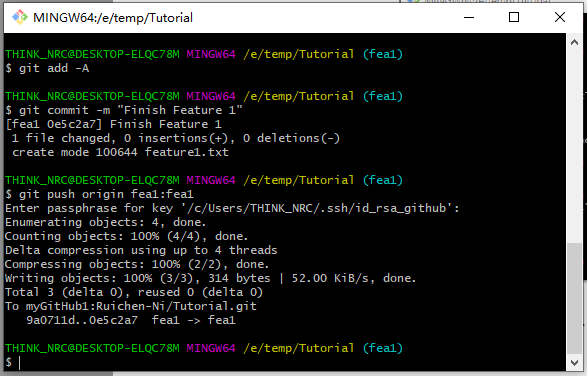
\includegraphics[height=6cm]{figure/step8}
\caption{将修改提交至远端仓库}
\end{figure}
\begin{figure}[h]
\centering
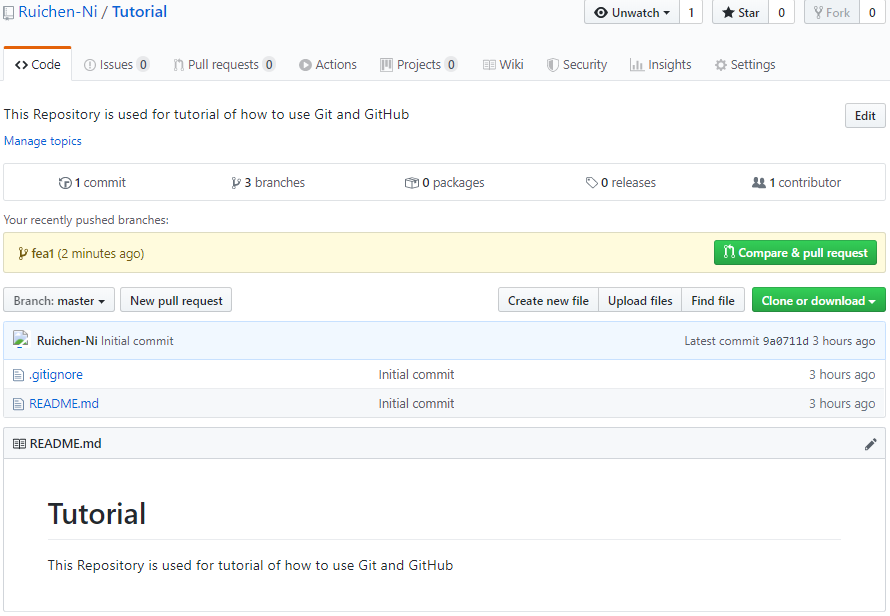
\includegraphics[height=9cm]{figure/step9}
\caption{发起Pull Request}
\end{figure}
\newpage
\item 如图28所示,A同学发起分支合并请求,在Tutorial软件的1.0版本开发过程中,我们需要将所有功能提交到dev开发分支上。等所有功能都开发完毕,再将dev分支合并到master分支上。(为了更有效地避免软件危机,可以对dev分支也设置和master分支一样的合并权限)填写完所有信息后点击“Create pull request”

\begin{figure}[h]
\centering
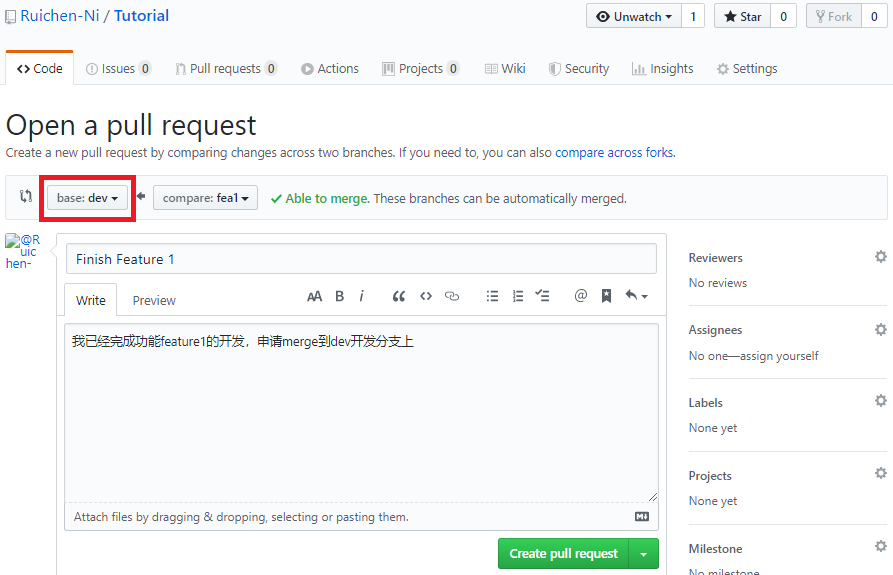
\includegraphics[height=9cm]{figure/step10}
\caption{发起Pull Request页面}
\end{figure}

\newpage
\item 如图29所示,A同学发起pull request后会进入一个类似投票的环节,如果有组员觉得添加的代码存在问题就可以在第三个红框上方的comment里写一段评论并关闭这次的pull request。A同学可以和那个组员进行在线comment argue,如果那个组员觉得A说的是对的,可以再重新reopen这个pull request,就像第一个红框操作的那样。如果在review界面(向设置了保护权限的分支合并时才会有进入该界面的链接,本例中的dev分支并没有设置保护权限。推荐给dev分支也设置权限保护)觉得添加的代码没问题就选择“Approve”,当认同的人数达到branch rule里设定的值时,第二个红框内的“merge pull request”按钮就会变得可以进行点击。

所有在GitHub远端的分支合并操作都会被记录下来,包括所有的comment信息。在大作业评分中我们会根据这个来判断大家的小组分工合作情况,所以请好好地撰写comment。
\begin{figure}[h]
\centering
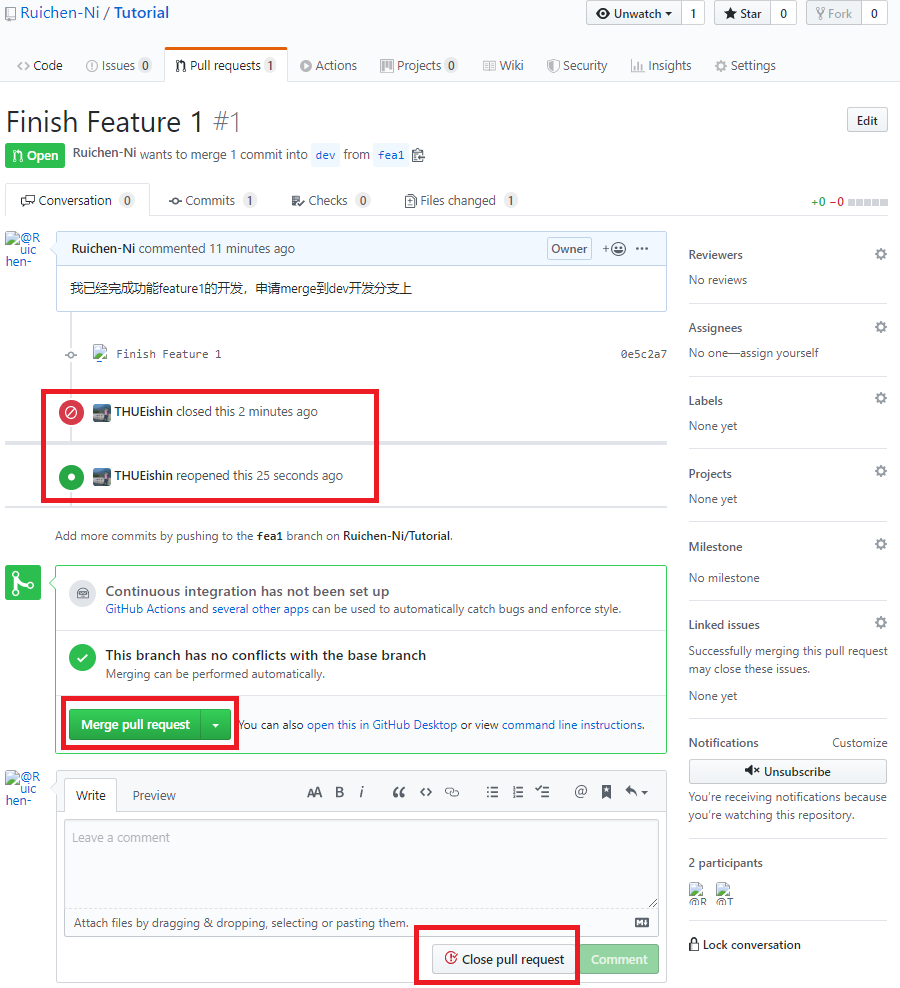
\includegraphics[height=16cm]{figure/step11}
\caption{组员决定是否进行merge}
\end{figure}

\newpage
\item 如图30所示,当merge成功后会出现该界面,由于feature1已经完成开发了,我们可以点击红框内的按钮删除fea1分支。
\begin{figure}[h]
\centering
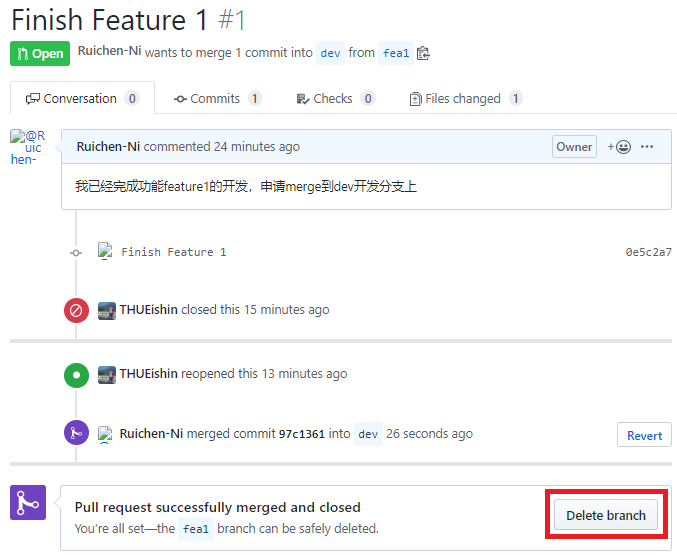
\includegraphics[height=10cm]{figure/step12}
\caption{成功merge并删除fea1分支}
\end{figure}
\item A同学在GitHub远端仓库merge的时候没有遇到冲突,所以在本地仓库也可以将fea1分支简单地合并到dev分支中,保持本地与远端的同步。相关命令如下
{\color{red}
\begin{lstlisting}[language=C]
git checkout dev     #切换回dev分支
git merge fea1         #将fea1分支merge到dev分支
git branch -d fea1    #删除fea1分支
git fetch origin dev   #从GitHub远端仓库获取dev的更新
git merge origin/dev  #将fetch到的远端分支克隆与本地的dev分支合并
\end{lstlisting}
}
\begin{figure}[h]
\centering
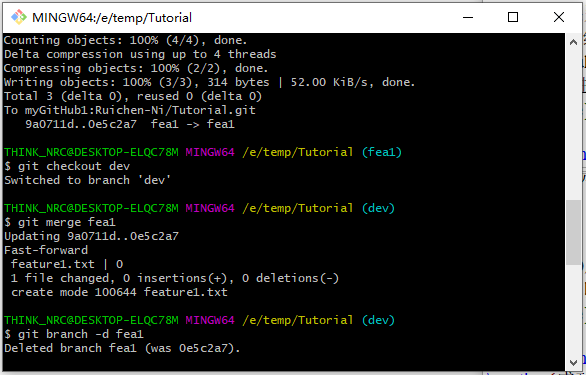
\includegraphics[height=6cm]{figure/step13}
\caption{切换分支、分支合并和删除分支}
\end{figure}
\begin{figure}[h]
\centering
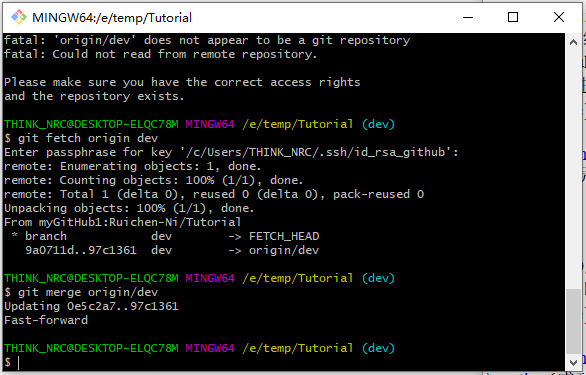
\includegraphics[height=6cm]{figure/step14}
\caption{保持本地分支和远端仓库分支同步}
\end{figure}
\end{enumerate}

\newpage
A同学已经完成了自己的工作,但是B同学的工作由于比较难还没有完成,A同学就开始帮助B同学检查B同学前面的代码是否有错误。而B同学就继续自己工作的代码撰写。我们希望通过这个案例来讲解分支合并冲突产生后的处理。

\begin{enumerate}[1. ]
\item 在A同学完成远端仓库的开发分支dev的创建后,B同学将远端仓库克隆到了本地准备开始feature2的开发。但是此时B同学本地只有master分支,并没有远端仓库的dev分支的克隆,因此B同学需要通过以下命令用远端仓库的dev分支创建本地dev分支。然后类似地创建fea2分支进行feature2的开发
{\color{red}
\begin{lstlisting}[language=C]
git checkout -b dev origin/dev
git checkout -b fea2
touch feature2.txt
git push origin fea2:fea2
\end{lstlisting}
}
\begin{figure}[h]
\centering
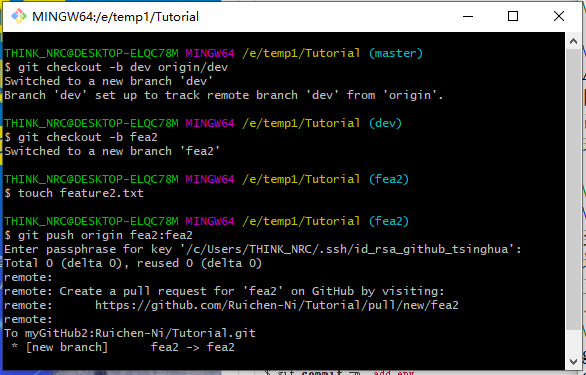
\includegraphics[height=6cm]{figure/stepB1}
\caption{本地dev分支创建、fea2分支创建和远端fea2分支创建}
\end{figure}

\newpage
\item B同学的feature2代码开发到一半,如图34所示。并通过如下命令将开发到一半的代码推送到GitHub远端仓库的fea2分支中进行代码保存以防代码丢失。
{\color{red}
\begin{lstlisting}[language=C]
git status
git add -A
git commit -m "Feature2 : Half"
git push origin fea2:fea2
\end{lstlisting}
}
\begin{figure}[h]
\centering
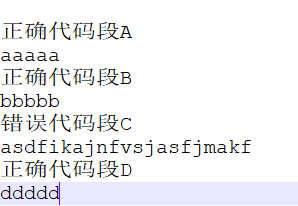
\includegraphics[height=3cm]{figure/stepB2}
\caption{B同学开发到一半的feature2代码}
\end{figure}
\begin{figure}[h]
\centering
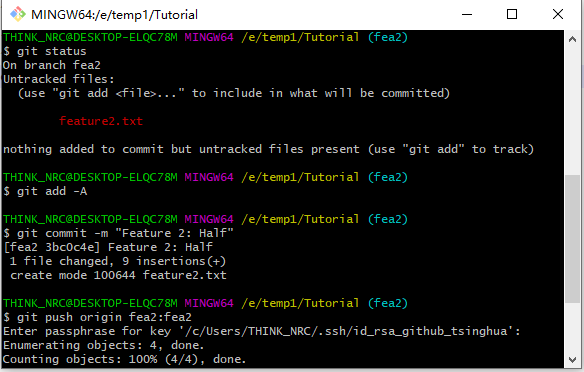
\includegraphics[height=6cm]{figure/stepB3}
\caption{B同学将开发到一半的feature2代码推送到远端仓库进行保存}
\end{figure}

\item A同学在此时加入帮助B同学debug前面的代码段,通过以下代码获取远端仓库的fea2分支,并从fea2分支上创建本地debug分支。
\begin{figure}[h]
\centering
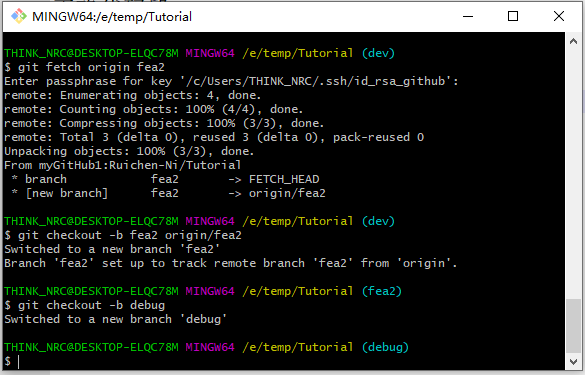
\includegraphics[height=6cm]{figure/stepB4}
\caption{获取远端仓库的fea2分支}
\end{figure}
{\color{red}
\begin{lstlisting}[language=C]
git fetch origin fea2
git checkout -b fea2 origin/fea2
git checkout -b debug
\end{lstlisting}
}

\item A同学在debug分支中找到了错误代码段C,并将其改正如图37所示。并切换回fea2分支,将debug分支上的修改merge到fea2分支上,然后将本地fea2分支推送到GitHub远端仓库的fea2分支。
{\color{red}
\begin{lstlisting}[language=C]
git status
git add -A
git commit -m "Debug: feature 2"
git checkout fea2
git merge debug
git branch -d debug
git pull origin fea2
git push fea2:fea2
\end{lstlisting}
}
\begin{figure}[h]
\centering
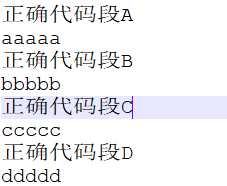
\includegraphics[height=3cm]{figure/stepB5}
\caption{修改代码}
\end{figure}
\begin{figure}[h]
\centering
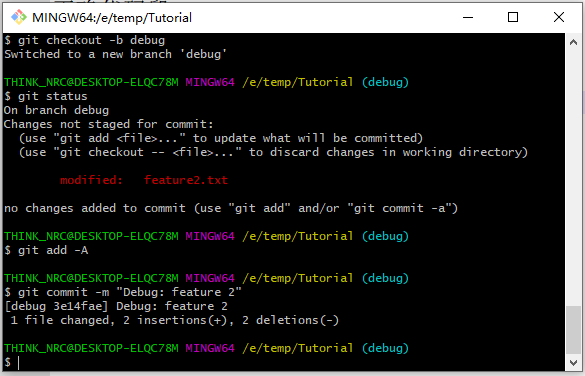
\includegraphics[height=6cm]{figure/stepB6}
\caption{修改bug并提交debug分支}
\end{figure}
\begin{figure}[h]
\centering
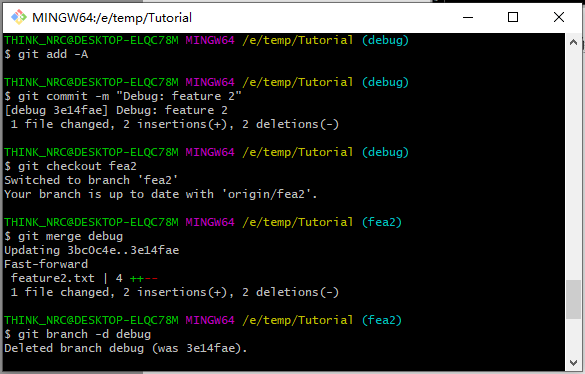
\includegraphics[height=6cm]{figure/stepB7}
\caption{将debug分支merge到fea2分支中}
\end{figure}
\begin{figure}[h]
\centering
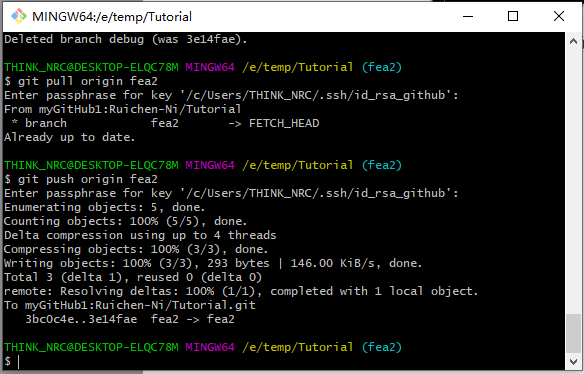
\includegraphics[height=6cm]{figure/stepB8}
\caption{将本地fea2分支推送到远端仓库的fea2分支中}
\end{figure}
\newpage
\item 此时B同学发现他写的代码段B和代码段C对实现feature2没有作用,就将其删除,最后feature2的代码如图41所示
\begin{figure}[h]
\centering
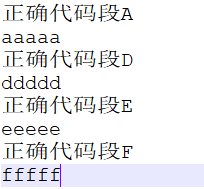
\includegraphics[height=3cm]{figure/stepB9}
\caption{feature2的最终代码}
\end{figure}

\item B同学通过如下命令将feature2的代码提交至本地fea2分支
{\color{red}
\begin{lstlisting}[language=C]
git status
git add -A
git commit -m "Finish Feature 2"
\end{lstlisting}
}
\begin{figure}[h]
\centering
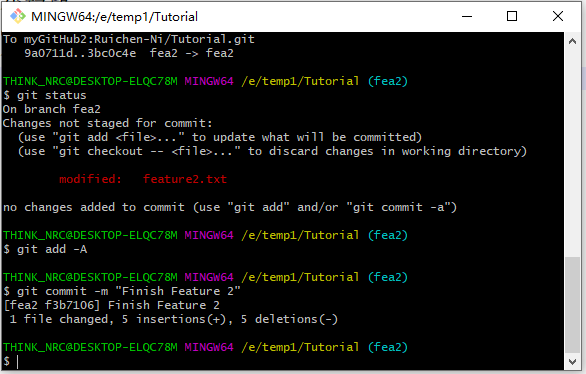
\includegraphics[height=6cm]{figure/stepB10}
\caption{将代码修改提交至本地fea2分支}
\end{figure}

\newpage
\item B同学的版本控制习惯较差,直接进行了git push命令,由于有其他用户在B同学之前向远端fea2分支进行过推送,因此被系统拒绝直接进行push。
{\color{red}
\begin{lstlisting}[language=C]
git push origin fea2
\end{lstlisting}
}
\begin{figure}[h]
\centering
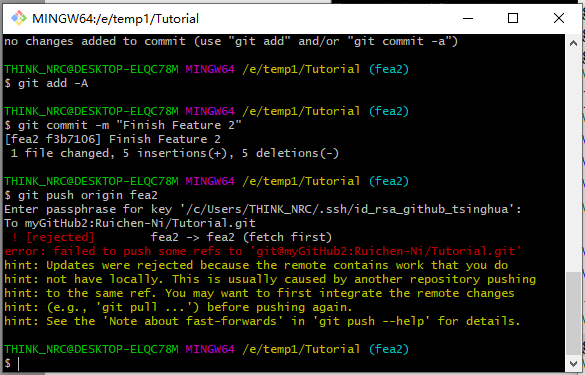
\includegraphics[height=6cm]{figure/stepB11}
\caption{向远端仓库的推送被拒绝}
\end{figure}

\item 因此B同学进行了git pull的操作,系统提醒存在内容冲突如图44所示。打开代码文件feature.txt可以看到相应的冲突
{\color{red}
\begin{lstlisting}[language=C]
git pull origin fea2
\end{lstlisting}
}
\begin{figure}[h]
\centering
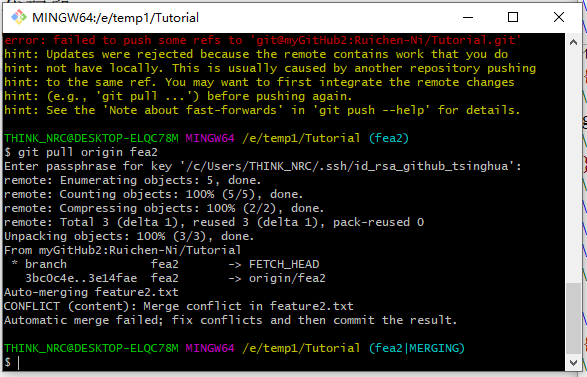
\includegraphics[height=6cm]{figure/stepB12}
\caption{git pull后系统提醒存在内容冲突}
\end{figure}
\begin{figure}[h]
\centering
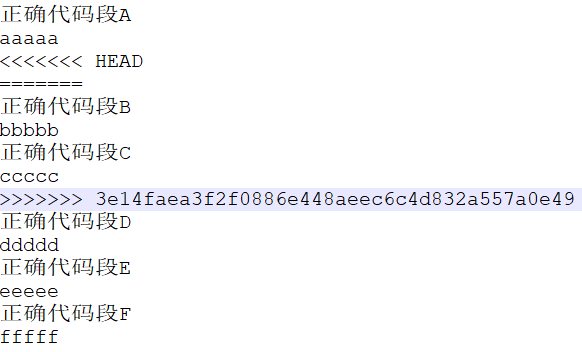
\includegraphics[height=4cm]{figure/stepB13}
\caption{出现冲突的内容}
\end{figure}

\newpage
\item 手动将feature.txt的文件修改为如图41所示,就可以通过如下命令将本地fea2分支推送至远端仓库的fea2分支。
{\color{red}
\begin{lstlisting}[language=C]
git status
git add -A
git commit -m "Fixed Conflict"
git push origin fea2
\end{lstlisting}
}
\begin{figure}[h]
\centering
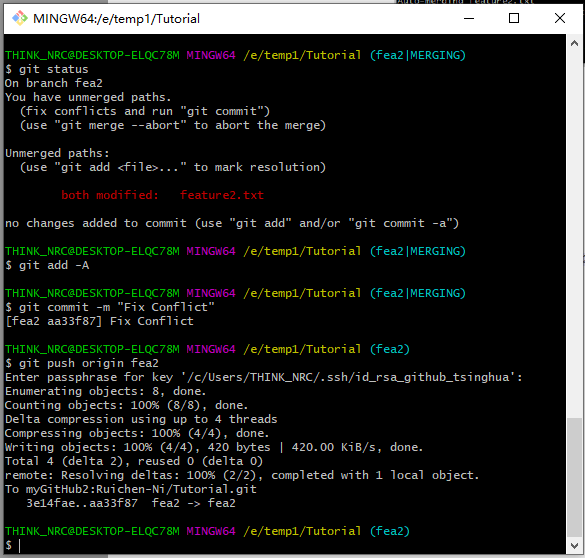
\includegraphics[height=10cm]{figure/stepB14}
\caption{解决冲突后重新推送本地的fea2分支}
\end{figure}

\item 类似A同学向master分支合并fea1分支一样,将fea2分支合并到dev分支中。由于所有功能都开发完毕了,所以我们可以将dev分支合并到master分支中完成1.0版本的Tutorial软件。如果再有任务要求添加新的功能更新软件的2.0版本,可以按这种方式进行软件迭代。
\end{enumerate}

\section{Git桌面版图形界面}
在这里给大家推荐两种界面简洁好用的桌面版图形界面:Sourcetree和GitKraken。由于Sourcetree只能在Windows和Mac OS系统下进行安装而助教的PC是Ubunutu系统,所以这里给大家重点介绍跨平台的GitKraken软件。

\subsection*{软件安装}
大家前往官网\url{https://www.gitkraken.com/}即可下载安装。

\newpage
\subsection*{软件的简单使用教程}

\quad

\begin{enumerate}[1.]
    \item 第一次运行软件会进入如图47所示的界面进行用户注册,我们选择第一项“Sign in with GitHub”,然后会自动跳转到GitHub网页进行授权操作。按照提示正常操作即可。
    \begin{figure}[h]
        \centering
        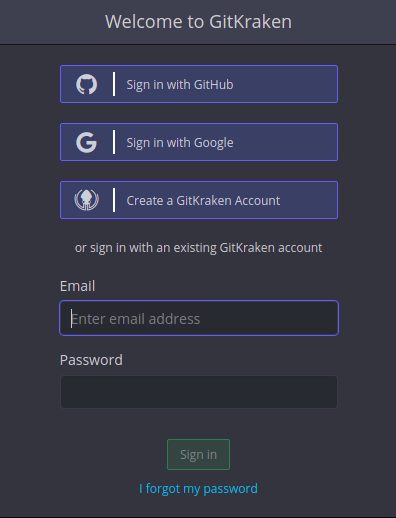
\includegraphics[height=5cm]{figure/GitKraken_sign.png}
        \caption{GitKraken软件的用户注册}
    \end{figure}

    \quad

    \item 授权完成后会进入到如图48所示的界面填写个人的相关信息,大家如实填写即可。
    \begin{figure}[h]
        \centering
        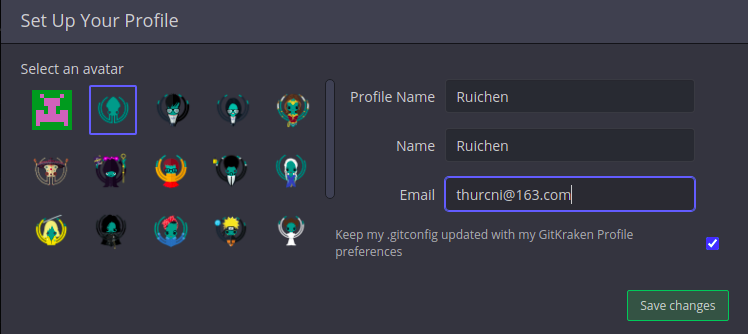
\includegraphics[height=6cm]{figure/GitKraken_profile.png}
        \caption{GitKraken软件的用户信息}
    \end{figure}
    
    \item 填写完上述信息以及以后打开GitKraken软件就会进入如图49所示的欢迎界面。
    
    \begin{figure}[htbp]
        \centering
        \includegraphics[height=8cm]{figure/GitKraken_start.png}
        \caption{GitKraken软件的欢迎界面}
    \end{figure}

    \item 我们点击图49中的“Clone a repo”的按钮就会进入到如图50所示的仓库克隆界面。由于我们在第一步的时候已经使用GitHub平台对GitKraken软件进行了授权,因此当我们选择列表中的“GitHub.com”时可以直接选择账号中的远端仓库,非常方便。当然也可以使用“Clone with URL”,将远端仓库的URL地址复制进去进行克隆。
    \item 成功克隆之后会在软件上方弹出如图51所示的弹窗,我们直接点击就能进入仓库的管理界面如图52所示。

    \begin{figure}[htbp]
        \centering
        \includegraphics[height=8cm]{figure/GitKraken_clone.png}
        \caption{GitKraken软件的仓库克隆界面}
    \end{figure}

    \begin{figure}[htbp]
        \centering
        \includegraphics[height=1cm]{figure/GitKraken_open.png}
        \caption{GitKraken软件的仓库克隆界面}
    \end{figure}

    \begin{figure}[htbp]
        \centering
        \includegraphics[height=8cm]{figure/GitKraken_repo.png}
        \caption{GitKraken软件的仓库管理界面}
    \end{figure}
\end{enumerate}

\newpage
\section{小结&作业}
\begin{enumerate}[1. ]
\item 请大家两人一组进行上述简单例子的实验熟悉Git版本控制和GitHub平台;
\item 请大家百度搜索《廖雪峰的Git教程》进行深入学习掌握Git版本控制的相关概念;
\item 请大家自行熟悉GitKraken图形界面,多尝试一下各个按钮以及各个位置处鼠标右键的下拉菜单。可以尝试使用GitKraken软件来完成上述的简单例子。
\item 希望大家牢记常用的Git命令。
\end{enumerate}
\end{document}
